\documentclass{article}
\usepackage[utf8]{inputenc}
\usepackage{multicol}
\usepackage{geometry}
\usepackage{multirow}
\usepackage{booktabs}
\setlength{\columnsep}{30pt} 
\usepackage{frontespizio}
\usepackage[T1]{fontenc}
\usepackage[utf8]{inputenc}
\usepackage{amsfonts}
\usepackage{amsmath}
\usepackage{bm}
\usepackage{empheq}
\usepackage{csquotes}
\usepackage[backend=biber,sorting=none]{biblatex} 
\usepackage{lipsum}
\usepackage{listings}
\usepackage[font=small,labelfont=bf]{caption}
\usepackage{url}
\usepackage[table]{xcolor}
\usepackage{float}
\usepackage[section]{placeins}
\graphicspath{ {./Figures/} }
\usepackage{graphicx,subfig,caption}
\usepackage{subfig}

\usepackage{algorithm,algorithmic}

\addbibresource{bibliography.bib}  

\usepackage{nicematrix}
\definecolor{codegreen}{rgb}{0,0.6,0}
\definecolor{codegray}{rgb}{0.5,0.5,0.5}
\definecolor{codepurple}{rgb}{0.58,0,0.82}
\definecolor{backcolour}{rgb}{0.95,0.95,0.92}







\geometry{margin=2cm}

\lstdefinestyle{mystyle}{
	backgroundcolor=\color{backcolour},
	commentstyle=\color{codegreen},
	keywordstyle=\color{magenta},
	numberstyle=\tiny\color{codegray},
	stringstyle=\color{codepurple},
	basicstyle=\ttfamily\footnotesize,
	breakatwhitespace=true,
	breaklines=true,
	captionpos=b,
	keepspaces=true,
	numbers=left,
	numbersep=8pt,
	showspaces=false,
	showstringspaces=false,
	showtabs=false,
	tabsize=2,
	breakindent=0pt ,
	columns=fullflexible,
	postbreak=\mbox{\textcolor{red}{$\hookrightarrow$}\space}
}



\lstset{breaklines=true}


\begin{document}
	
	
	\title{LSTM autoencoder for anomaly detection on ECG data}
	\author{R. Lorusso}
	\date{2023 - University of Bari Aldo Moro}
	
	\maketitle
	
	\begin{multicols*}{2}
		
		\section*{Abstract}
		\begin{it}
			The aim of this work is to provide a model for effectively identify anomalies in vital parameters time series selected from VitalDB dataset \cite{VitalDB}. The employed model is an LSTM autoencoder as a tool to identify anomalies in such temporal data by the evaluation of the mean reconstruction error.
			Furthermore an adaptive threshold selection based on the training data reconstruction error it's proposed, with the aim of improving the explainability of the model without relying on an arbitrary threshold.
			
			
		\end{it}
		
		
		
		\section{Introduction}
		
		The detection of anomalies, also known as outliers, is an integral practice across a diverse range of disciplines. Anomalies can indicate a breach of a system or network, signal abnormal physiological levels, or even flag the occurrence of fraud. Regardless of the particular application, analytics and machine learning models have the potential to provide both predictive and descriptive value. Anomaly detection can be used to inform about anomalous data that can be indicative of health complications. This kind of information can be very useful to professionals as a first insight to a possible patient problem. Since providing care and track patient vitals signals can be hard to maintain trough the time, machine learning can be very helpful by automatically detect rare deviations from normal data trends, thus providing health care professionals with useful information with which make more accurate and quicker clinical decisions. However what is to be considered as an anomaly isn't ever clearly defined. The main assumptions are that anomalies are infrequent an somehow they differ from normal data. Furthermore anomalies can differ substantially one from each other, thus introducing more uncertainty about their nature. Sometimes oscillations in the test data can be detected as anomalies, introducing false alarms. Especially in the e-health domain, we are interested in reducing or minimizing the number of false alerts, since an high false alarm rate can decrease the trust in the system and in the alarm itself.
		In order to cope with these problems, an adaptive threshold selection based on the mean reconstruction error on training data is proposed.
		In section \ref{model} we'll start with a formal definition of a general autoencoder and how it can be employed to identify anomalies. Section \ref{dataset} describes the dataset and its selected features through a preliminary exploratory data analysis. Then we can move to section \ref{preprocessing}, focusing our attention on the features and preprocessing strategy. Finally in section \ref{model_development} it's introduced the model implementation, which is further evaluated in section \ref{results} by means of the obtained results.
		
		\section{Employed model}
		\label{model}
		Autoencoders are widely used for anomaly detection tasks in a variety of different fields and for many purposes. 
		The choice of an LSTM autoencoder is motivated by the use of time series in health domain \cite{VitalDB}.
		An autoencoder is a feed forward neural networks used to learn a latent representation of unlabeled input data and it is trained to reconstruct the input at the output layer.
		Autoencoders are made by an encoder and a decoder, which can be described by two maps $\Phi$  and $\Psi$ on $X \in \Re^n$, $Y \in \Re^d$, $d < n$ such as:
		\begin{align*}
			\Phi : X \rightarrow  Y \\
			\Psi : Y \rightarrow  X  
		\end{align*}
		for which the goal is to minimize the mean squared error between the input and the output layer
		\begin{equation*}
			argmin_{\Phi,\Psi}|| X -  (\Psi  o \Phi) X ||^2.
		\end{equation*}
		The main assumption is that the data fed to the model in the training phase is to be considered normal.
		Since the neural network encodes an input data point in a latent space learned from normal data, and decodes it from the very same space to reconstruct its original form, we can evaluate the degree of fitness to the model by measuring the reconstruction error through a distance metric.  If the reconstruction error is large enough,  then we can assume that the tested sample can be considered an anomaly since it doesn't fit the latent space, being different from the training data.
		
		\begin{figure}[H]
			\centering
			\subfloat{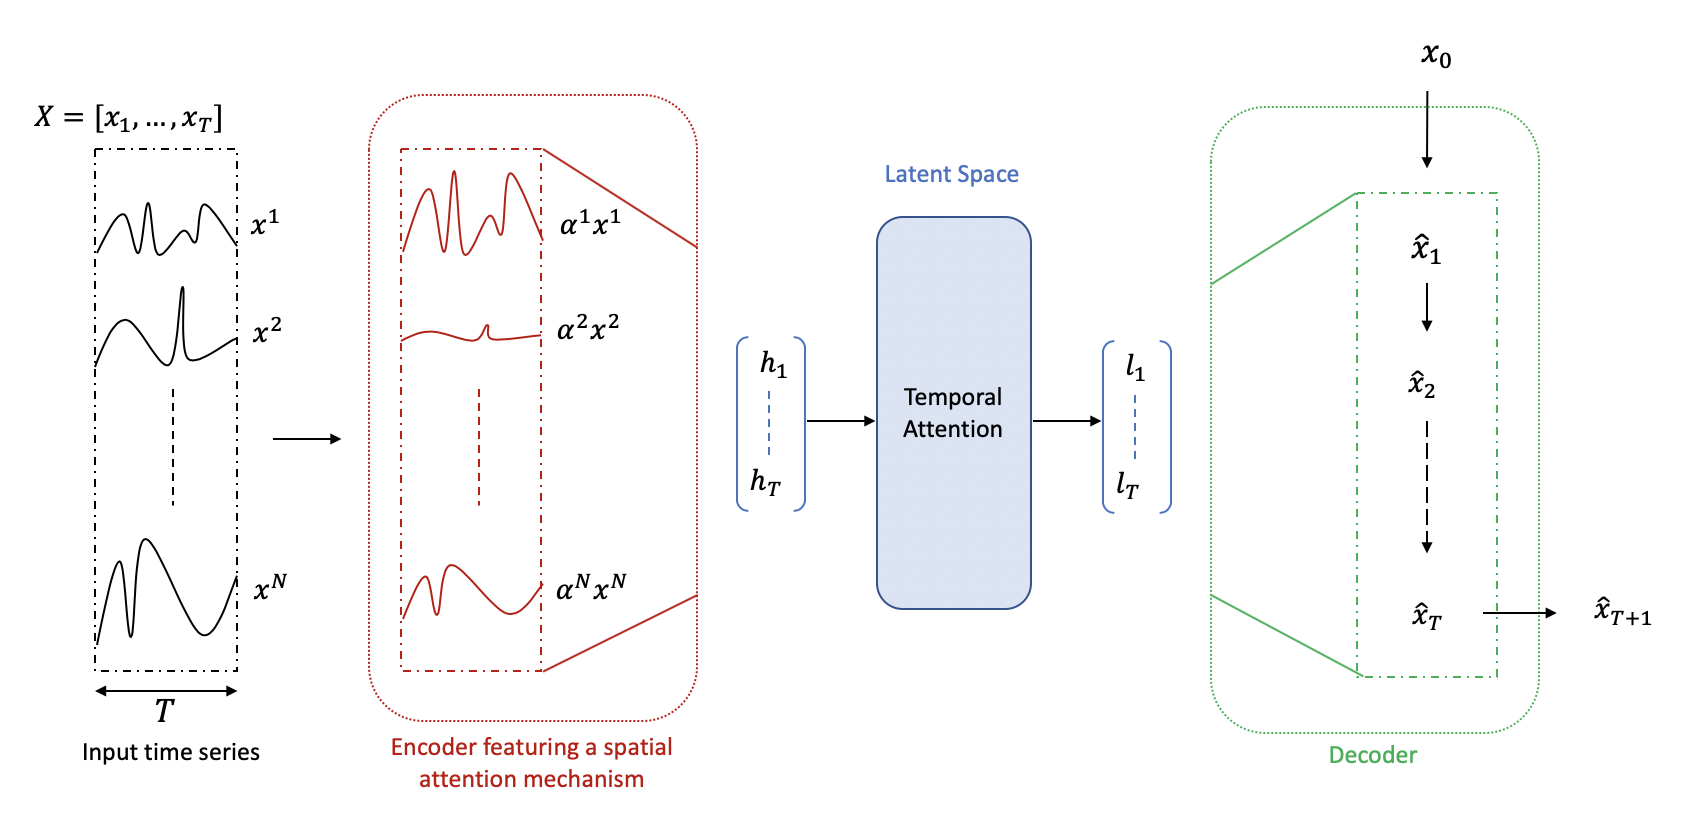
\includegraphics[width=0.9\linewidth]{imgs/autoencoder.png}\label{fig:autoencoder}}
			\caption{General autoencoder architecture}
		\end{figure}
		
		\section{Dataset Description}
		\label{dataset}
		The dataset employed is called VitalDB \cite{VitalDB}, it contains high-resolution multi-parameter data from 6,388 cases of surgical patients. The mean age of the patient is 57 years.
		Among the plethora of different features, the following have been selected:
		\begin{itemize}
			\setlength\itemsep{-0.1em}
			\item Diastolic blood pressure,
			\item Systolic blood pressure,
			\item Body temperature,
			\item Heart rate,
			\item Respiratory rate,
		\end{itemize}
		which are the basic vital parameters, useful for a first assessment of a patient health state.
		Since the dataset contains records of vital parameters of surgical patient, the ones with the most healthiest values have been selected by means of the ASA physical status system \cite{ASA}.
		Only those records with an ASA grade less than three are retained for training the model, resulting in the distribution depicted in the diagram \ref{fig:raw_data}.
		A percentage of this data is held out for testing and evaluating the model, which will be used further for detecting anomalies on the portion of dataset with ASA equal to three i.e. "patients with severe systemic disease".
		From diagram \ref{fig:raw_data1} it's possible to observe how the distribution of such data it's more irregular and slightly shifted to the right side of the chart for the first three parameter, while for the distribution of respiratory rate and body temperature values is very similar.
		\begin{figure}[H]
			\centering
			\subfloat[ASA  <  3]{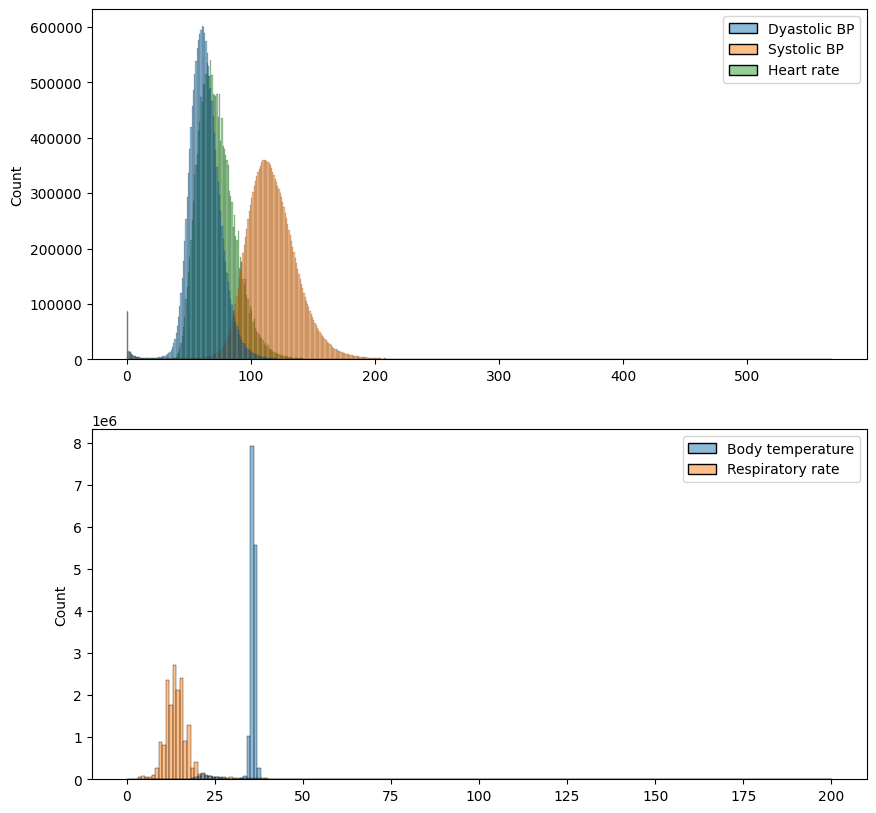
\includegraphics[width=0.6\linewidth]{imgs/raw_data.png}\label{fig:raw_data}}
			\subfloat[ASA == 3]{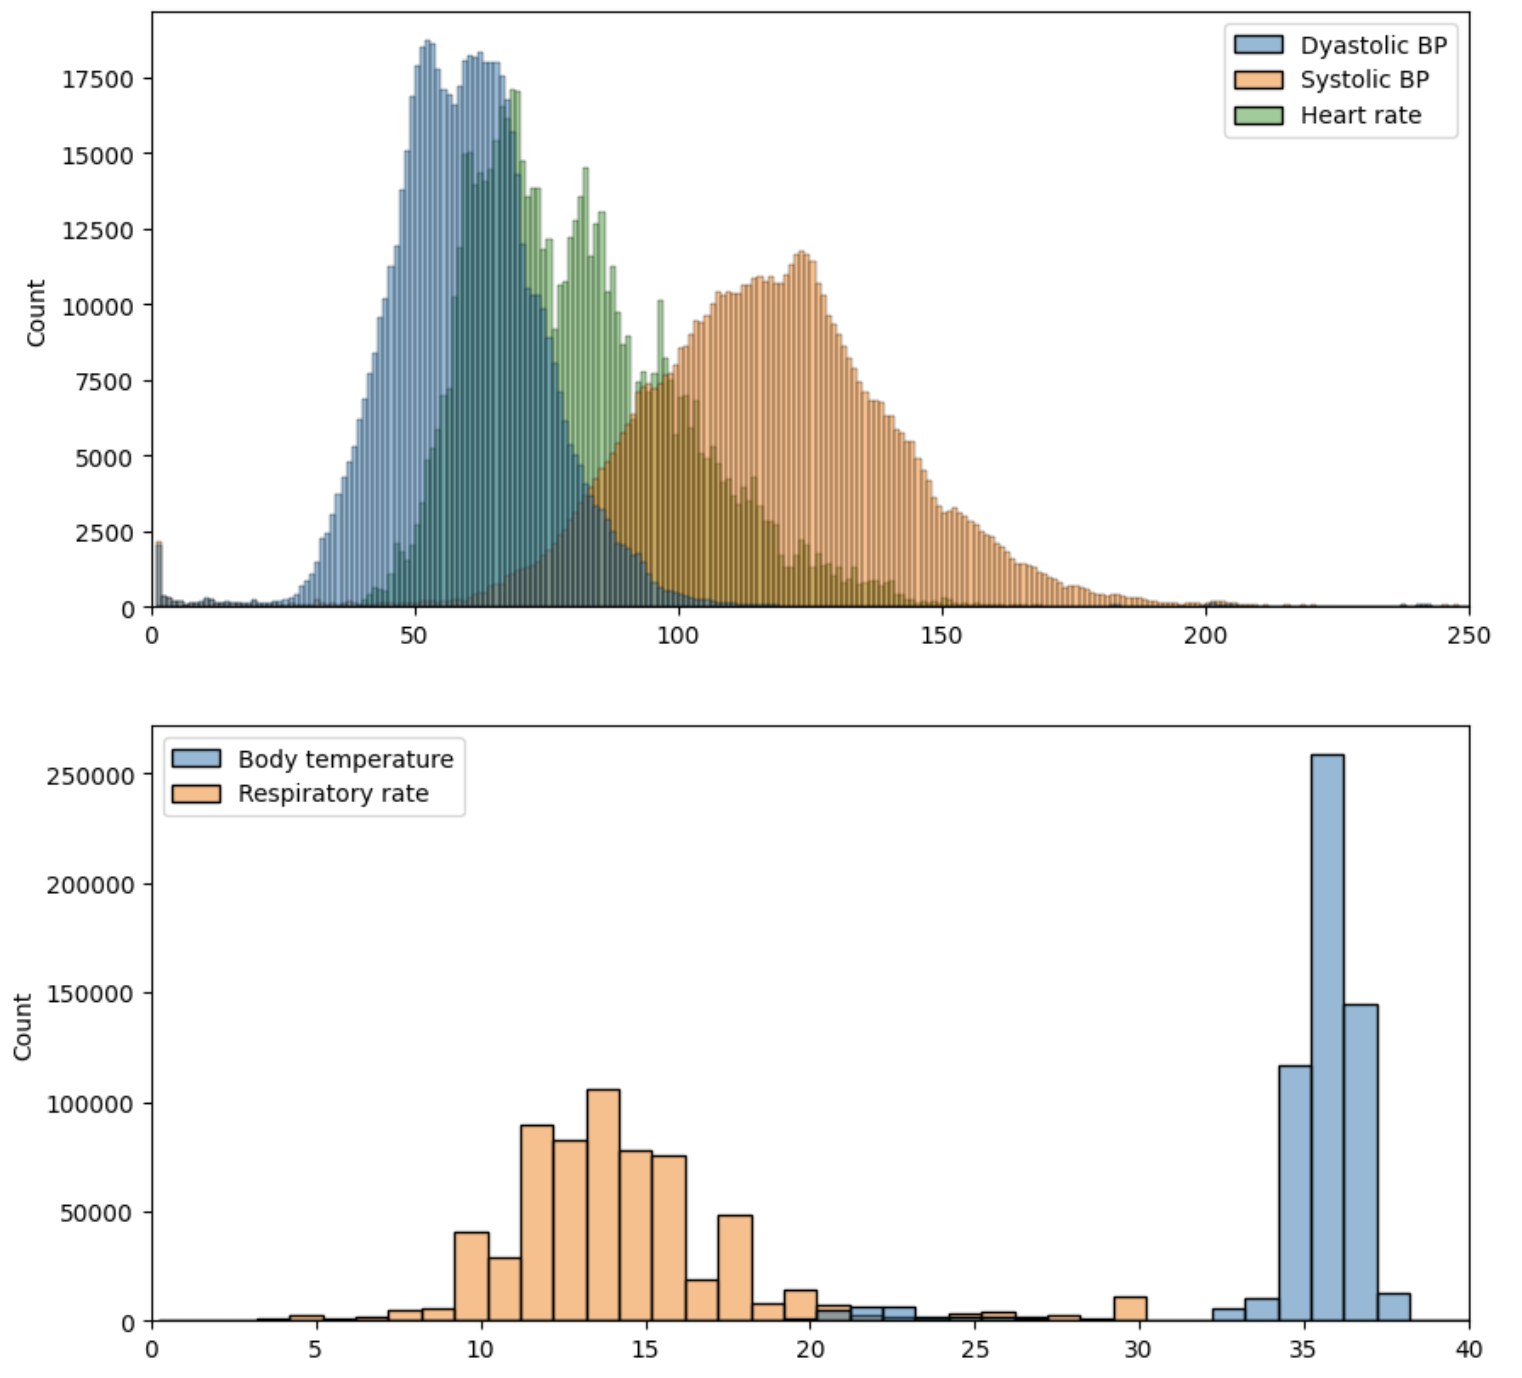
\includegraphics[width=0.6\linewidth]{imgs/asa_eq_3.png}\label{fig:raw_data1}}
			\caption{Data distribution}
		\end{figure}
Since every feature presents anomalous values, the following section describes the preprocessing strategy applied to retain only the features values which can be considered normal.
Before going into details of the preprocessing strategy it's worth to notice that the data has been collected from surgical patients during a perioperative period \cite{VitalDB}. Considering this context it is possible to deduce that the results obtained by a model trained on such data could be useful in the same kind of context but may be wrong in another one, such as during physical activity. We will talk about this in the section \ref{ethics} related to the ethical issues.
\section{Feature Engineering}
		\label{preprocessing}
As anticipated, it has been needed to retain only the features values which can be considered healthy. This is done by following both common knowledge, as in the case of body temperature, and international approved guidelines \cite{ESC} as in the case of the blood pressure.

\subsection{Data cleaning}
Every feature records have been cleaned from NaN and negative values, which where consistently present into the data. Then time series are cleaned from values outside the following ranges:
		\begin{itemize}
			\item Diastolic blood pressure: 40-100;
			\item Systolic blood pressure: 85-140;
			\item Body temperature: 35-37.2;
			\item Heart rate: 40-120;
			\item Respiratory rate: 8-22.
		\end{itemize}
These range values are a bit wider than the optimal ones to preserve some variability and noise in the data without making the model too rigid in detecting anomalies. However restricting the data in a range can introduce sudden changes in time series values, thus negatively affecting its quality. To partially overcome this problem, the values outside a range are replaced with the mean value of the sample; a better solution would be that of interpolation for smoothing the gap between two values.
		
After restricting the values in ranges by replacing the outsiders with the sample mean, we obtain a new data distribution depicted in the diagram \ref{fig:clean_data}. Wider data intervals will result in a loosen anomaly detection.
\begin{figure}[H]
			\centering
			\subfloat{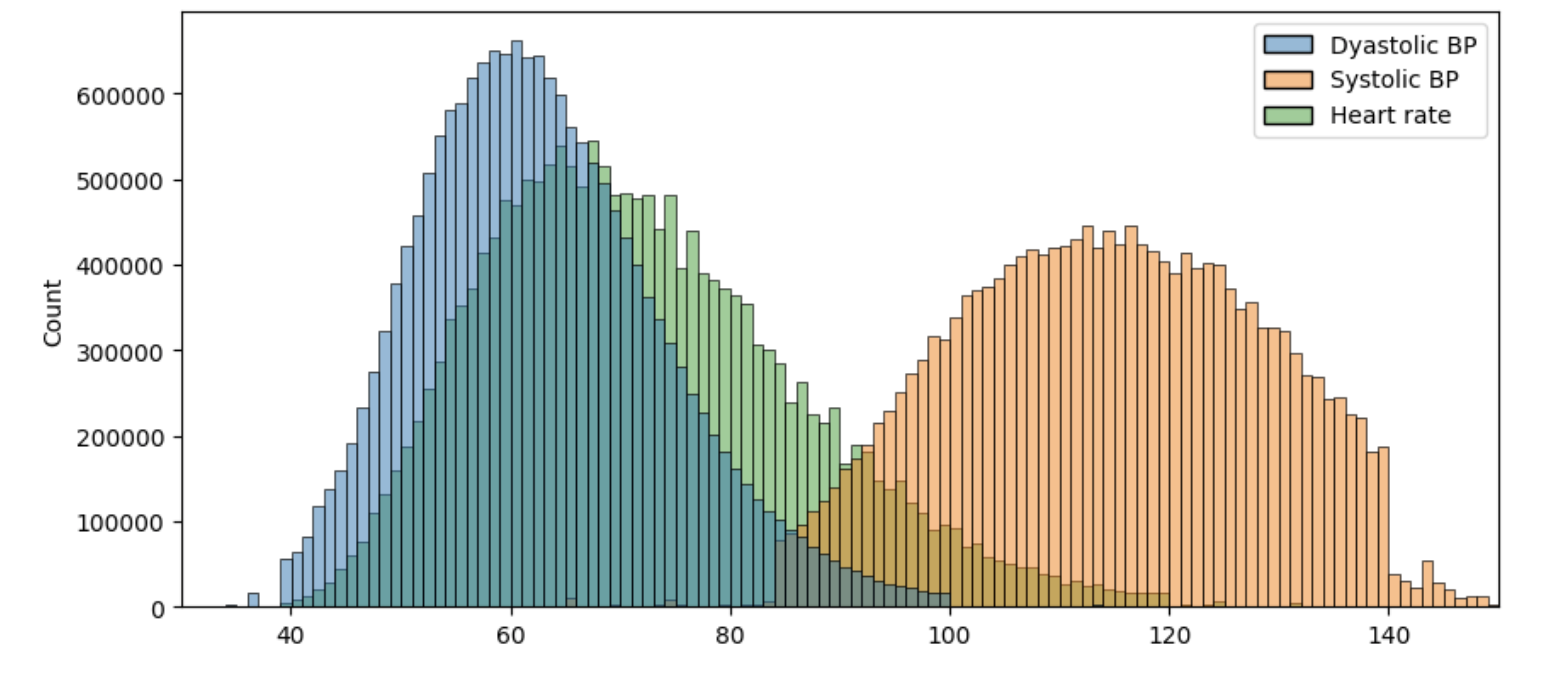
\includegraphics[width=0.5\linewidth]{imgs/clean_data.png}\label{fig:clean_data}}
			\subfloat{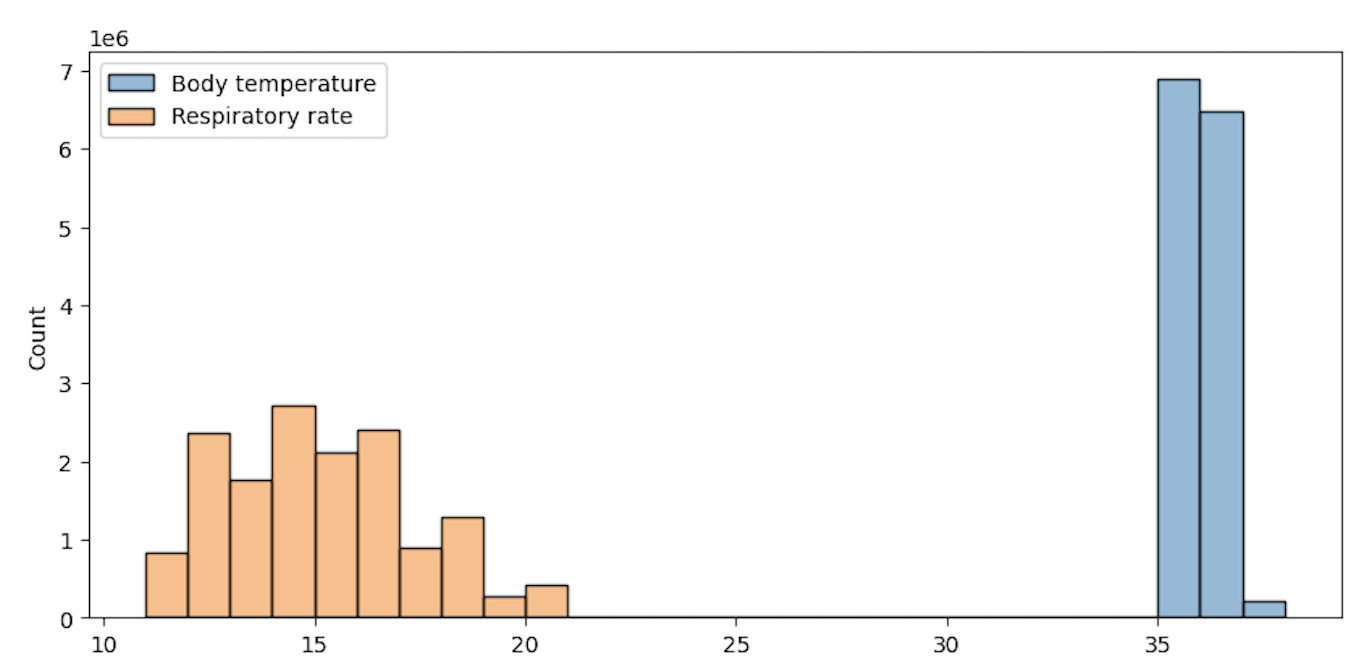
\includegraphics[width=0.5\linewidth]{imgs/bt_rr_clean.png}\label{fig:bt_rr_clean}}
			\caption{Data distribution restricted to ranges}
\end{figure}
As ultimate step, it is removed every record which is either empty or has negative mean since vital parameters can't have negative values nor be null.
		
\subsection{Data bundling and chunking}
After the data has been cleansed from anomalous values, the time series along the different features are concatenated to create a unique one. This big sequence is then chunked into ones of equal length to be fed to the model.
Since feature values follow a normal distribution, a Std normalization has been applied.

\section{Model development}
\label{model_development}
The model employed for this task is a multivariate LSTM autoencoder, the choice is motivated by the time series data. It is implemented using Keras library.
By the moment that we are in a semi-supervised context since we are selecting the data by means of the ASA parameter, has been possible to hold out a part of the data in order to evaluate the model performances on such testing data.
In diagram \ref{fig:model} is depicted the model architecture. As we can see from the input shape, the time series length is equal to 4678. This value can be diminished on enlarged to carry out a more local or global analysis respectively. In this case the input shape is selected as the minimum length of the records across the different features.

\begin{figure}[H]
	\centering
	\subfloat{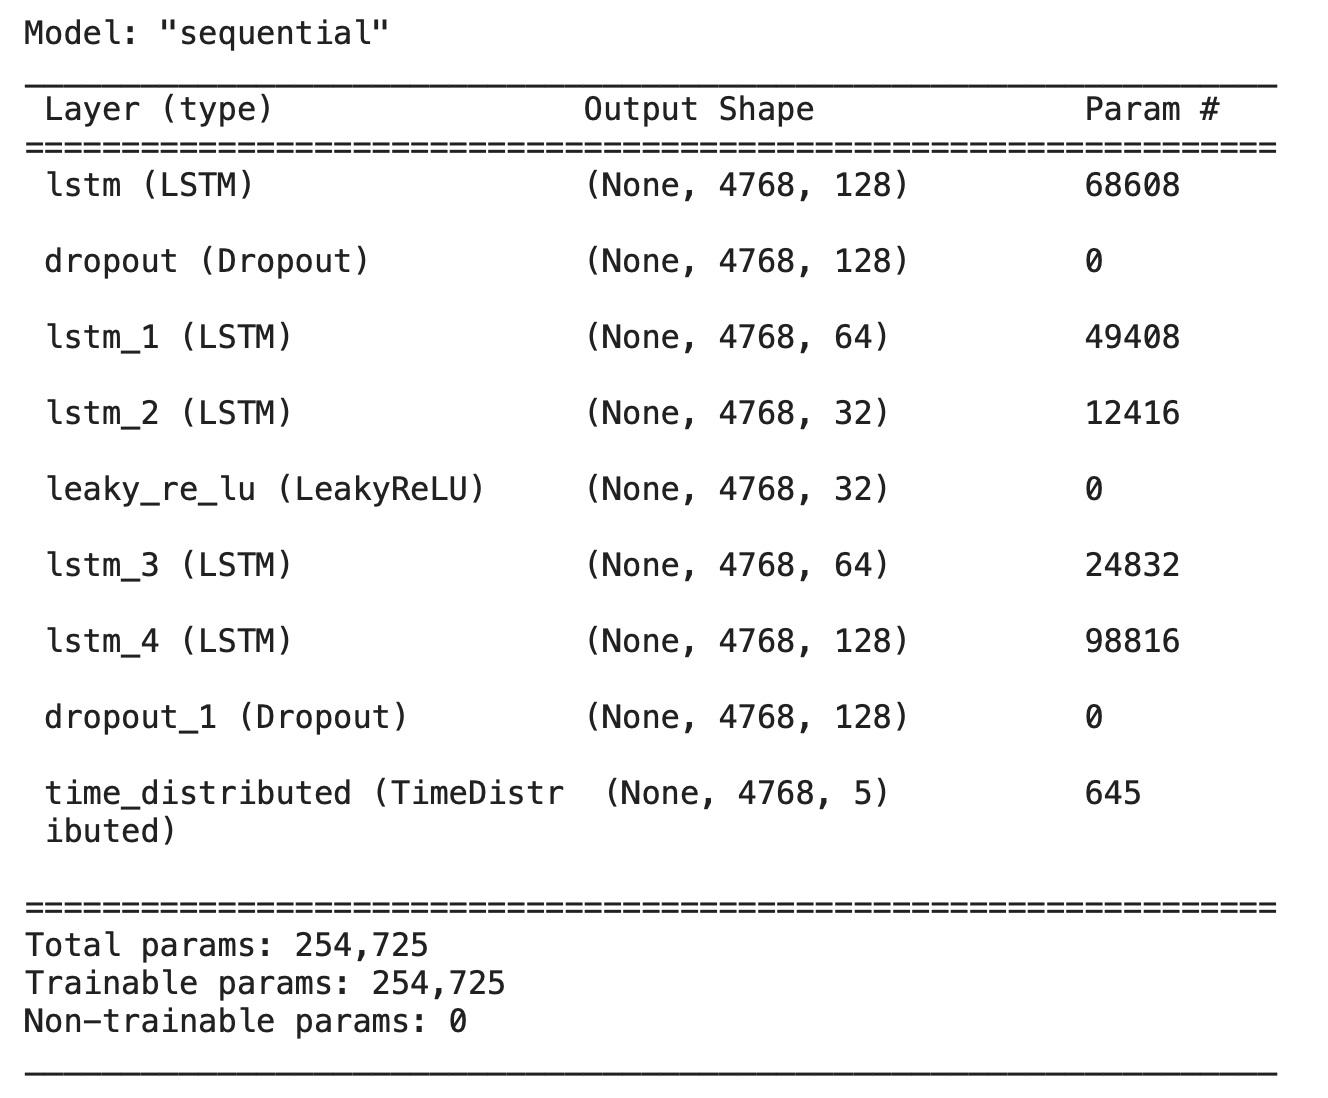
\includegraphics[width=0.6\linewidth]{imgs/model.png}\label{fig:model}}
	\caption{LSTM autoencoder architecture}
\end{figure}

\subsection{Configuration} 
The final configuration of the parameters has been obtained after several training sessions.
The best results are yielded with the following parameter settings: 
\begin{itemize}
	\item epochs = 50;
	\item loss function =  Mean Squared Error;
	\item bias regularizer = 0.3;
	\item recurrent regularizer = 0.1;
	\item batch\_size = 64;
	\item validation split = 0.1.
\end{itemize}

The 80\% of data with ASA less than three is retained for training and the remaining 20\% is held out for testing.
In section \ref{results} it is showed a comparison between the mean reconstruction errors made on the training and testing data in order to see if the model behaves as expected by producing a similar mean reconstruction error for the two sets.

\section{Adaptive threshold selection}
As already discussed in the introduction, identification of anomalies relies on the assumption that these are rare and differ from normal data. In the context of autoencoders an anomaly is detected evaluating the reconstruction error by means of a threshold, manually left to the human. Most of the times threshold value is decided by looking to the distribution of reconstruction errors, although recent studies propose standard deviation based methods to adapt such value \cite{adaptivethresh}.
In this section is described a simple approach to adapt the threshold by means of the mean reconstruction error made by the autoencoder on training data. Given the reconstruction error for all the training sample it is possible to select the threshold value which encloses a given percentage of data below such value. Since we are interested to identify anomalies, we can start by the mean reconstruction error made on the training set and increment it until the above condition si met.


\begin{algorithm}[H]
\caption*{Adaptive threshold selection}
\begin{algorithmic}
	\STATE $X$ \COMMENT{Autoencoder input, array of time series}
	\STATE $Y$ \COMMENT{Autoencoder output, array of time series}
	\STATE $n\_samples \gets len(X)$ 
	\STATE $mean\_rec\_err $ \COMMENT{Train set mean reconstruction err}
	\STATE $target \gets 0$
	\STATE $percentage \gets .98$
	\STATE $step \gets 1 - percentage$
	\STATE $factor \gets 1 - step$
	
	\WHILE{target < percentage}
			\STATE $j \gets 0$
				\STATE $factor \gets factor + step$
				
				\FOR{i in  range(0,n\_samples)}
					\STATE $err \gets norm2(X[i] - Y[i])$
					\IF{$err \le mean\_rec\_err \times factor$)}
					\STATE $j \gets j+1$
					\ENDIF
				\ENDFOR
			\STATE$target \gets j \div n\_samples$
	\ENDWHILE\
	
	\STATE $threshold \gets factor \times mean\_rec\_err$
\end{algorithmic}
\end{algorithm}
		
\section{Experimental results}
\label{results}
		
		
\section{Related Works}
		
\section{Ethical issues and opportunities}
		\label{ethics}
		
\nocite{*}
\printbibliography
		
		
	\end{multicols*}
	
\end{document}





